\documentclass[12pt, twoside]{article}
\usepackage{jmlda}
\usepackage[]{algorithmic}
\usepackage{graphicx}
\usepackage{multicol}
\usepackage{caption}
\graphicspath{{../figures}}
\usepackage{subfig}
\newcommand{\hdir}{.}
\epstopdfsetup{outdir=./}
\newtheorem{statement}{Утверждение}

\begin{document}

\title
    []
    {Мультиязычный тематический поиск и категоризация научных публикаций}

\author
    [Е.\,В.~Тищенко]
    {Е.\,В.~Тищенко, К.\,В.~Воронцов}
    [Е.\,В.~Тищенко$^1$, К.\,В.~Воронцов$^2$, П.\,С.~Потапова$^3$]

\abstract{
В статье рассматривается задача кроссязычного поиска текстового плагиата. Целью работы является получение модели, выделяющей информацию о распределении слов в тексте независимо от их языковой принадлежности, при этом ограниченной по размеру и времени обучения для ее практического использования.

\textbf{Ключевые слова}: \emph{машинное обучение, тематическое моделирование, мультиязыковой поиск дубликатов, обработка текстов на естественном языке, мультиязыковая обработка текстов}
}



\maketitle
\linenumbers
\section{Введение}

Задача поиска и распознавания тематически близких документов является важной из-за невозможности проверить все документы общей тематики на плагиат в силу размеров глобальной сети. Задача становится особенно трудной, так как возникает множество документов, являющихся переводом исходных работ. Согласно исследованиям Donald L. McCabe,\cite{donaldSurvey}  $ 36\% $ студентов американских университетов перефразировали или копировали информацию из всемирной паутины без ссылки на источник. 

Методы векторизации документов для поиска плагиата  \cite{methodMLPlag, regression} преимущественно ограничиваются одним языком. В таком случае возникает проблема создания единообразной системы получения векторных представлений мультиязыковой коллекции документов. Для возможности применения модели за пределами научных экспериментов ставятся технические ограничения ресурсами сервера, а именно на размер модели, временную сложность обучения.

Объектом исследования являются мультиязыковые тематические модели, алгоритмы поиска документов в текстовой коллекции по словам и документам, способы векторного представления слов и документов запроса и коллекции, применяемые для поиска дубликатов независимо от языковой принадлежности.

Тематическая модель коллекции текстовых документов определяет, к каким темам относится каждый документ и какие слова или термины образуют каждую тему. Вероятностная тематическая модель описывает каждую тему дискретным распределением вероятностей слов, а каждый документ $\--$ дискретным распределением вероятностей тем. Тематическая модель преобразует любой текст в вектор вероятностей тем. 

Для решения задачи используется мультимодальная тематическая модель. Такая тематическая модель описывает документы, содержащие метаданные наряду с основым текстом. Под метаданными подразумеваются языковая принадлежность документа, авторство, дата публикации, ссылки на иные источники и многое другое. Метаданные улучшают точность определения тематики документа. В качестве модальностей используются 100 языков, а также научные рубрики Государственного рубрикатора научно-технической информаци (ГРНТИ)\footnote{grnti.ru} и Универсального десятичного классификатора (УДК)\footnote{udcsummary.info}. Использование языков в качестве модальностей позволяет получить векторное представление текста, независимое от оригинального языка текста, что позволяет решать проблему поиска плагиата без ограничения на язык статьи. Во время предобработки текста используется BPE токенизация $\--$ итеративная замена наиболее встречаемой пары символов на символ, который не встречается в слове. Это существенно уменьшает объем изначального словаря для практического применения модели.

Целью эксперимента является построение модели, исследование влияния регуляризации и предобработки текстовых данных на качество поиска, подбор разнообразных функций для сравнения тематических расстояних векторов а также поиск эвристик для улучшения точности предсказаний модели. В качестве обучающих данных используются статьи с сайта Wikipedia, а также выборка научных статей из научной электронной библиотеки eLIBRARY.ru.

\section{Постановка задачи поиска дубликатов документов}

Пусть $D~-$ некоторая коллекция документов, $T~-$ множество тем документов. Кандидатом на дубликат  для документа $d \in D$ обозначим такой элемент коллекции $f(d)$, что  $$f(d) = \argmin_{d' \in D \setminus \{d\}} distance(m(d), m(d'))$$ 
В качестве функции $distance$ может быть использована произвольная метрика векторного пространства. Функция  $m(d) \--$ модель, осуществляющая преобразование документа в векторное пространство. Качество модели поиска дубликатов измеряется на тестовой выборке при помощи двух метрик сопоставления документов:

1. Средняя частота, с которой документ-запрос попадает в топ 10\%.  Для документа в тестовой выборке уже известно, какие документы являются переводом исходного. Рассматривается доля тех документов, для которых среди 10\% отранжированных кандидатов на дубликат встречаются их переводы. 

2. Средний процент документов в топ 10\% документов-переводов, которые имеют такую же рубрику, что у документа-запроса. Аналогично предыдущей метрике, однако рассматриваются доля тех документов, для которых наиболее близкими в векторном представлении оказываются документы той же рубрики.

Требуется решить задачу поиска дубликатов, при этом качество должно превосходить 0.9 по первой метрке, 0.3 по второй. Также необходимо ограничить размер модели до 100 Гб, а обучение модели должно производиться не более чем за 24 часа.

В качестве преобразования текства в векторном представлении используется тематическое моделирование. Тематическая модель \cite{basetematic}  по коллекции документов строит вероятностное распределение $p(w|t)$ термов w $-$ слов, словосочетаний и терминов в темах $t \in T$. Согласно гипотезе об условной независимости, а также формуле полной вероятности, распределение термов w в документе d является вероятностной смесью распределений термов в темах $\phi_{wt} = p(w|t)$ с весами $\theta_{td}=p(t|d)$

$$p(w|d) = \sum_{t \in T} p(w|t, d)p(t|d) = \sum_{t \in T} p(w|t)p(t|d) =\sum_{t\in T}\phi_{wt}\theta_{td}$$

Данное выражение можно переписать в матричном виде. Матрица частот термов в документах $F \approx \Phi \Theta$. Так как число тем, как правило, намного больше, чем число документов, то требуется найти такое разложение, ранг которого не превосходит $|T|$.


\section{Вычислительный эксперимент}

В рамках эксперимента ставится задача поиска оптимальных параметров тематической модели, а также метода токенизации текста, при которых будут достигнуты требования на качество модели, а также физические ограничения. После выбора оптимальных параметров будет проведен абляционный эксперимент, показывающий вклад каждого отдельного решения на общее качество модели.

Стоит обратить внимание на то, каким образом генерируется тестовая выборка. Поиск тематически близкого документа осуществляется не по всей поисковой коллекции, а по подвыборке документов, в которой 10\% документов имеет такую же рубрику УДК, что и документ-запрос, а остальные 90\% документов имеют другую рубрику УДК.

\subsection{Данные}

В качестве данных для обучения тематической модели использовались статьи научной электронной библиотеки eLibrary\footnote{elibrary.ru}, а также статьи многоязычной интернет-энциклопедия Wikipedia\footnote{wikipedia.org}, описанные в работе \cite{}. % Как сослаться на статью, которую ещё не опубликовали?. 
Для подавляющего числа научных статей eLibrary были известны рубрики ГРНТИ и УДК. Формирование выборки статьей на 100 языках происходило следующим образом. Было отобрано 24 тысячи статей библиотеки eLibrary на русском и английском языках. Затем статьи были переведены на 42 языка. Языки были выбраны по причине их большой представленности среди научных текстов. Перевод осуществлялся при помощи системы статистического машинного перевода Moses \cite{Moses}. Также для всех языков, включая эти 42, были собраны статьи из энциклопедии Wikipedia.

Ниже представлено распределение обучающих данных по рубрикам УДК и ГРНТИ. Стоит отметить несбалансированность выборок по объему документов, что влечет проблемы при обучении, так как предполагается обучать модель на сбалансированных данных. Кроме того среди рубрик ГРНТИ присутствует рубрика <<нет>>, которая представляет набор документов, не принадлежащих к другим рубрикам. Данная рубрика содержит документы, относящиеся к различным темам и является четвертой по размеру среди всех рубрик.

\begin{figure}[h]
  \subfloat{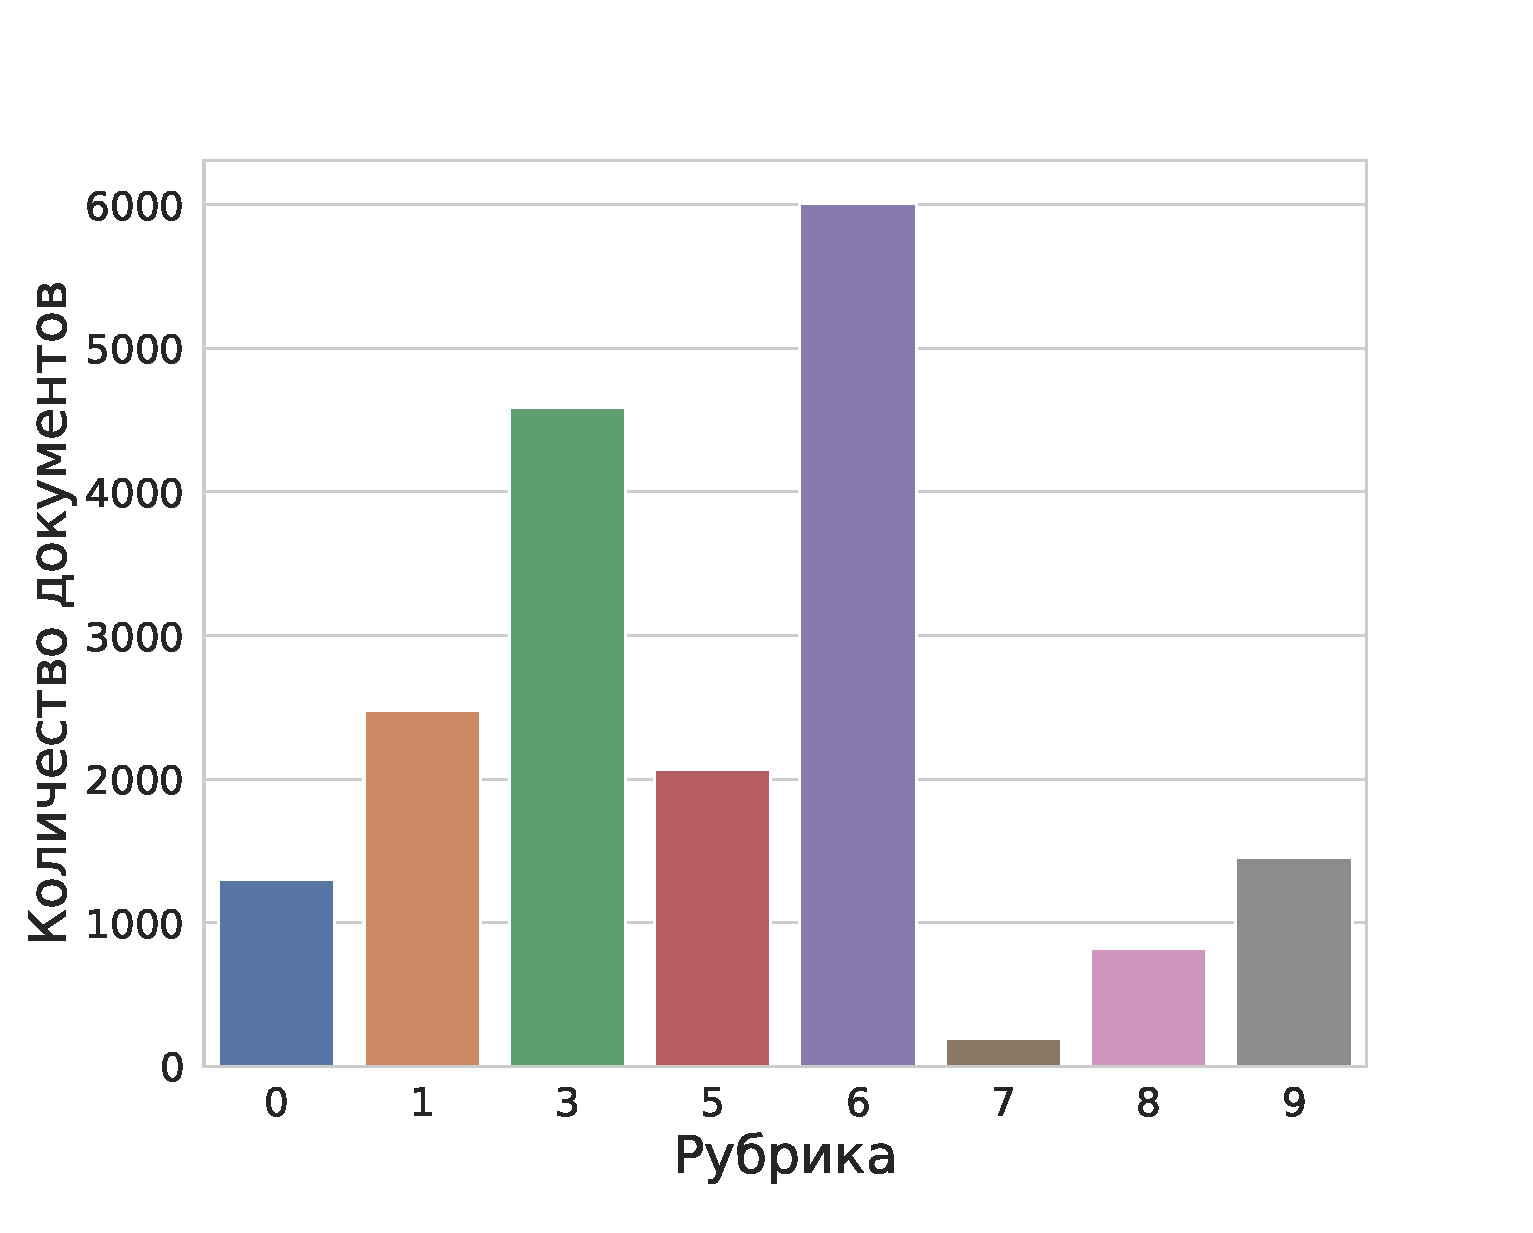
\includegraphics[width=0.5\textwidth]{udk.eps}}
  \subfloat{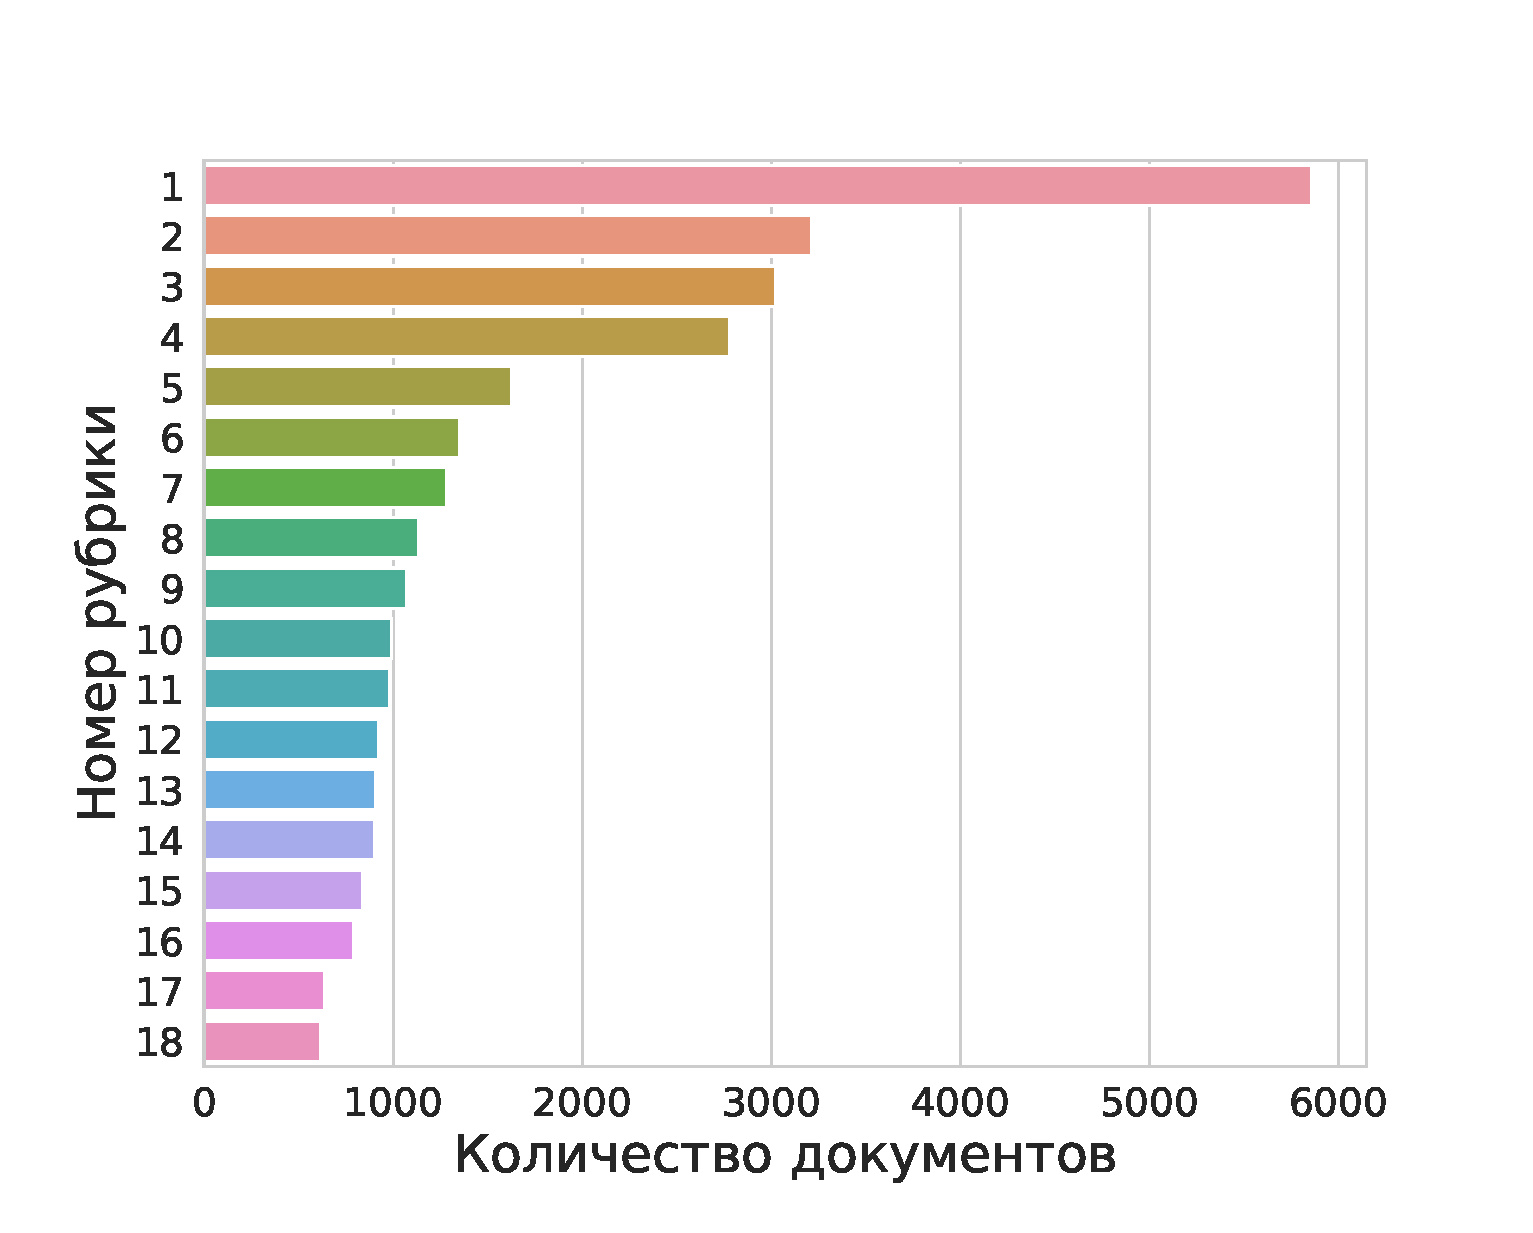
\includegraphics[width=0.5\textwidth]{grnti.eps}}
 \caption{Распределение данных по рубрикам УДК и ГРНТИ}
  \label{fig:1}
\end{figure}

\subsection{Базовые модели}

В качестве базовой модели используется тематическая модель, использующая в качестве модальностей 100 языков. Обучение происходит на основе данных Википедии. Используются 300 тем, из них одна является фоновой. Фоновая тема содержит все общеупотребимые слова, не являющиеся предметными. К ним относятся предлоги, частицы, союзы и другие неинформативные части речи. При предобработке текста используется метод BPE токенизации, причем изначальный объем словаря в 120 тысяч токенов ужат до 2 тысяч для каждого отдельного языка. Обучение модели занимает порядка 6 часов, а размер модели составляет 4.6 Гб. 

Также в качестве еще одной базовой модели рассматривается нейросетевая модель XLM-RoBERTa. Описание появится позже.

\section{Предложенное решение}

Применение к базовой тематической модели различных эвристик, а также поиск оптимальных параметров позволяет добиться требуемых результатов. При обучении модели подбирается оптимальное количество тем в промежутке от 10 до 1000. Наилучшие результаты были достигнуты при выделении 125 отдельных тем. Существенный прирост вносит добавление модальностей рубрик УДК и ГРНТИ. 

Обучение тематической модели происходит итеративно, на каждой итерции отбирается случайная подвыборка документов. Для решения проблемы несбалансированности данных относительно рубрик, на каждой итерации обучения генерируется подвыборка документов, для которой распределение рубрик ГРНТИ оказалось равномерным. Таким образом, в каждой подвыборке документов количество документов с различными рубриками одинаково.

Уменьшение словаря до 2 тыс. токенов на язык позволяет учесть ограничения на размер модели, однако такого количества токенов недостаточно для описания отдельного языка. Использование 11 тыс. токенов позволяет не только улучшить выразительность модели, а значит ее качество, но и соблюдать ограничения на время обучения, которое составляет не более 24 часов.

Использование рубрики <<нет>> снижает качество модели, так как в ней представлены документы различной тематики. Для повышения качества модели принято решение не учитывать эту рубрику и не устанавливать ее в качестве модальности для документов. Помимо этого решено исключить стоп-слова из 15 основных языков.

Обучение занимает 25 итераций, на рис. 2 представлено, как изменяется метрика средняя частота ГРНТИ в зависимости от номера итерации.

\begin{figure}[h]
\centering
  \subfloat{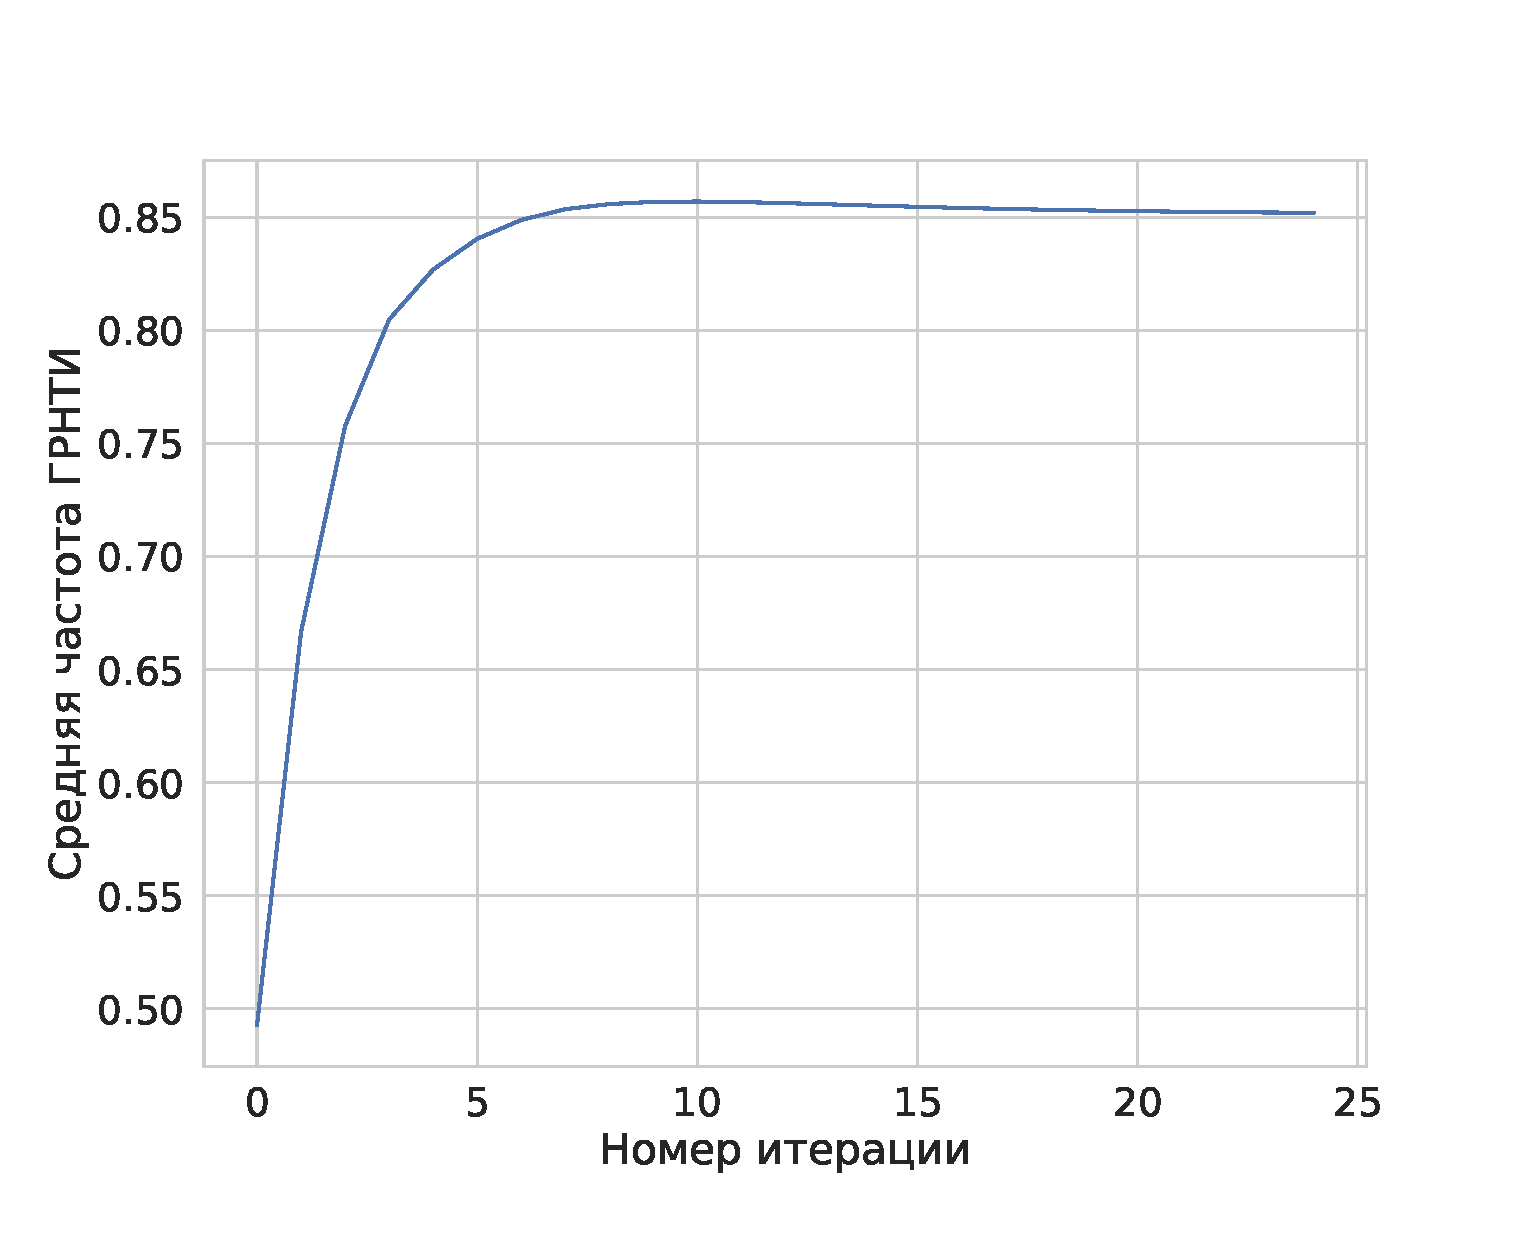
\includegraphics[width=0.5\textwidth]{error.eps}}
 \caption{Средняя частота ГРНТИ в зависимотси от итерации обучения}
  \label{fig:1}
\end{figure}

\subsection{Результаты}

Ниже представлено сравнение базовых решений с итоговым.

\begin{table}[h]
\centering
\begin{tabular}{|c|c|c|c|c|}
\hline
\textbf{Название модели}     & \begin{tabular}[c]{@{}c@{}}Средняя \\ частота\\ УДК\end{tabular} & \begin{tabular}[c]{@{}c@{}}Средний \\ процент\\ УДК\end{tabular} & \begin{tabular}[c]{@{}c@{}}Средняя \\ частота\\ ГРНТИ\end{tabular} & \begin{tabular}[c]{@{}c@{}}Средний\\ процент\\ ГРНТИ\end{tabular} \\ \hline
Базовая тематическая модель  & 0.5584                                                           & 0.1652                                                           & 0.5364                                                             & 0.2196                                                            \\ \hline
XLM-RoBERTa                  & Coming                                                           & Coming                                                           & Coming                                                             & Coming                                                            \\ \hline
Итоговая тематическая модель & 0.995                                                            & 0.225                                                            & 0.852                                                              & 0.366                                                             \\ \hline
\end{tabular}
\end{table}

\subsection{Абляционные эксперименты}

\begin{thebibliography}{4}

\bibitem{donaldSurvey}
    \BibAuthor{Donald L. McCabe}
    Cheating among college and university students: A North American perspective//
    \BibJournal{International Journal for Educational Integrity}, 2005
    
\bibitem{methodMLPlag}
    \BibAuthor{Zdenek Ceska, Michal Toman, and Karel Jezek}
    Multilingual Plagiarism Detection//
    \BibJournal{Artificial Intelligence: Methodology, Systems and Applications}, 2008
    
\bibitem{regression}
    \BibAuthor{Duygu Ataman, Jose G. C. de Souza, Marco Turchi, Matteo Negri}
    Cross-lingual Semantic Similarity Measurement Using Quality Estimation Features and Compositional Bilingual Word Embeddings//
    
\bibitem{basetematic}
    \BibAuthor{Воронцов К. В.}
    Обзор вероятностных тематических моделей.//
  
\bibitem{Moses}
  \textit{Koehn P. et al.} Moses: Open source toolkit for statistical machine translation //Proceedings of the 45th annual meeting of the association for computational linguistics companion volume proceedings of the demo and poster sessions. – 2007. – С. 177-180.

	  
\end{thebibliography}

\end{document}




% Ищем на подвыборке: 10% такая же научная рубрика УДК 90%, . Среди такой такой выборки ищем перевод.